\documentclass[3p, authoryear, review]{elsarticle} %review=doublespace preprint=single 5p=2 column
%%% Begin My package additions %%%%%%%%%%%%%%%%%%%
\usepackage[hyphens]{url}

  \journal{Journal of Transportation and Land Use} % Sets Journal name


\usepackage{lineno} % add
\providecommand{\tightlist}{%
  \setlength{\itemsep}{0pt}\setlength{\parskip}{0pt}}

\usepackage{graphicx}
\usepackage{booktabs} % book-quality tables
%%%%%%%%%%%%%%%% end my additions to header

\usepackage[T1]{fontenc}
\usepackage{lmodern}
\usepackage{amssymb,amsmath}
\usepackage{ifxetex,ifluatex}
\usepackage{fixltx2e} % provides \textsubscript
% use upquote if available, for straight quotes in verbatim environments
\IfFileExists{upquote.sty}{\usepackage{upquote}}{}
\ifnum 0\ifxetex 1\fi\ifluatex 1\fi=0 % if pdftex
  \usepackage[utf8]{inputenc}
\else % if luatex or xelatex
  \usepackage{fontspec}
  \ifxetex
    \usepackage{xltxtra,xunicode}
  \fi
  \defaultfontfeatures{Mapping=tex-text,Scale=MatchLowercase}
  \newcommand{\euro}{€}
\fi
% use microtype if available
\IfFileExists{microtype.sty}{\usepackage{microtype}}{}
\usepackage{natbib}
\bibliographystyle{plainnat}
\usepackage{longtable}
\usepackage{graphicx}
\ifxetex
  \usepackage[setpagesize=false, % page size defined by xetex
              unicode=false, % unicode breaks when used with xetex
              xetex]{hyperref}
\else
  \usepackage[unicode=true]{hyperref}
\fi
\hypersetup{breaklinks=true,
            bookmarks=true,
            pdfauthor={},
            pdftitle={If you build it who will come? Equity analysis of park system changes during COVID-19 using passive origin-destination data},
            colorlinks=false,
            urlcolor=blue,
            linkcolor=magenta,
            pdfborder={0 0 0}}
\urlstyle{same}  % don't use monospace font for urls

\setcounter{secnumdepth}{5}
% Pandoc toggle for numbering sections (defaults to be off)

% Pandoc citation processing

% Pandoc header
\usepackage{booktabs}
\usepackage{longtable}
\usepackage{array}
\usepackage{multirow}
\usepackage{wrapfig}
\usepackage{float}
\usepackage{colortbl}
\usepackage{pdflscape}
\usepackage{tabu}
\usepackage{threeparttable}
\usepackage{threeparttablex}
\usepackage[normalem]{ulem}
\usepackage{makecell}
\usepackage{xcolor}
\usepackage{booktabs}
\usepackage{longtable}
\usepackage{array}
\usepackage{multirow}
\usepackage{wrapfig}
\usepackage{float}
\usepackage{colortbl}
\usepackage{pdflscape}
\usepackage{tabu}
\usepackage{threeparttable}
\usepackage{threeparttablex}
\usepackage[normalem]{ulem}
\usepackage{makecell}
\usepackage{xcolor}



\begin{document}
\begin{frontmatter}

  \title{If you build it who will come? Equity analysis of park system changes during COVID-19 using passive origin-destination data}
    \author[BYU]{Gregory S. Macfarlane\corref{1}}
   \ead{gregmacfarlane@byu.edu} 
    \author[Harvard]{Carole Turley Voulgaris}
   \ead{cvoulgaris@gsd.harvard.edu} 
    \author[StreetLight]{Teresa Tapia}
   \ead{teresa.tapia@streetlightdata.com} 
      \address[BYU]{Brigham Young University, Civil and Environmental Engineering Department, 430 Engineering Building, Provo, Utah 84602}
    \address[Harvard]{Harvard Graduate School of Design, 48 Quincy St, Cambridge, Massachussetts 02138}
    \address[StreetLight]{StreetLight Data, Inc., San Francisco, California}
      \cortext[1]{Corresponding Author}
  
  \begin{abstract}
  During the spring and summer of 2020, cities across the world responded to the global COVID-19 pandemic by converting roadway facilities into open pedestrian spaces. These conversions improved access to public open space, but measuring the variation in that improvement among different populations requires clear definitions of access and methods for measuring it. In this study, we evaluate the change in a utility-based park accessibility measure resulting from street conversions in Alameda County, California. Our utility-based accessibility measure is constructed from a park activity location choice model we estimate using mobile device data --- supplied by StreetLight Data, Inc.~--- representing trips to parks in that county. The estimated model reveals heterogeneity in inferred affinity for park attributes among different sociodemographic groups. We find, for example, that neighborhoods with more lower-income residents and those with more residents of color show a greater preference for park proximty while neighborhods with higher incomes and those with more white residents show a greater preference for park size and amenities. We then apply this model to examine the accessibility benefits resulting from COVID-19 street conversions to create a set of small park-like open spaces; we find that this policy has improved equity in that maginalized communities including Black, Hispanic, and low-income households receive a disproportionate share of the policy benefits, relative to the population distribution.
  \end{abstract}
   \begin{keyword} Accessibility Passive Data Location Choice Parks\end{keyword}
 \end{frontmatter}

\hypertarget{intro}{%
\section{Introduction}\label{intro}}

Parks and other open spaces generate immense value for the public who are able
to access them. The \citet{CityParksAlliance} categorizes the observed benefits of
urban parks as encouraging active lifestyles \citep{Bancroft2015}, contributing to
local economies, aiding in stormwater management and flood mitigation, improving
local air quality, increasing community engagement \citep{Madzia2018}, and enhancing
public equity.

For many, the value of public parks and open public spaces increased during the
widespread lockdowns enacted in 2020 to slow the transmission of COVID-19. With
other entertainment venues shuttered and people otherwise confined to their
homes, periodic use of public space provided an opportunity for physical and
emotional relief unavailable in other forms. Paired with this increased demand
for public open space --- and the with the epidemiological requirement to leave
sufficient space between other users --- was the related collapse in demand for
vehicular travel. As a result, cities around the world began closing select
streets to automobile travel, thereby opening them as pedestrian plazas, open
streets, or slow streets \citep{glaser_can_2021, schlossberg_rethinking_2021, combs2021shifting}. The effective result of this policy was to create a number
of ``parks'' in urban areas that may have had poor access previously.
Understanding the equitable distribution of these benefits is an important land
use policy issue. The potential for non-emergency temporary or permanent street
conversions also brings up interesting problems for land use and transportation
policy; indeed, the possibility for transportation infrastructure to \emph{become} a
socially beneficial land use that goes beyond serving mobility needs is a
tantalizing proposition.

Unfortunately, quantifying the benefits derived from access to parks in general
is a complicated problem. Many previous attempts at quantifying access in terms
of isochronal distances or open space concentration have resulted in a
frustrating lack of clarity on the relationship between measured access and
measures of physical and emotional health \citep{Bancroft2015}. Central to this
confusion is the fact that people do not always use the nearest park, especially
if it does not have qualities that they find attractive. A better methodology
would be to evaluate the park activity location choices of people in a
metropolitan area to identify which features of parks --- distance, amenities,
size, etc. --- are valued and which are less valued. The resulting activity
location choice model would enable the evaluation of utility benefits via the
choice model logsum \citep{Handy1997, DeJong2007}.

In this study, we seek to evaluate the socio-spatial distribution of benefits
received by residents of Alameda County, California resulting from the
temporary conversion of streets to public open spaces during the spring and
summer of 2020. We estimate a park activity location choice model using
location-based services (LBS) data obtained through StreetLight Data, Inc., a
commercial data aggregator. The resulting model illuminates the degree to which
simulated individuals living in U.S. Census block groups of varying
sociodemographic characteristics value the walking distance between their residence
and parks, the size of the parks, and the amenities of parks including sport
fields, playgrounds, and walking trails in Alameda county. We then apply this
model to examine the inferred monetary benefit resulting from the street
conversion policy, and its distribution among different sociodemographic groups.

The paper proceeds in the following manner: A \protect\hyperlink{literature}{discussion} of prior
attempts to evaluate park accessibility and preferences is given directly. A
\protect\hyperlink{methodology}{Methodology} section presents our data gathering and cleaning
efforts, the econometric framework for the location choice model, and the
approach taken to apply the models to analyze open streets projects. A
\protect\hyperlink{results}{Results} section presents the estimated choice model coefficients
alongside a discussion of their implications, including the implied benefits
resulting from the street conversions in Alameda County. After presenting
\protect\hyperlink{limitations}{limitations} and associated avenues for future research, a final
\protect\hyperlink{conclusions}{Conclusions} section outlines the contributions of this study for
recreational trip modeling and location choice modeling more generally.

\hypertarget{literature}{%
\section{Literature}\label{literature}}

Understanding the equity benefit distribution of park access requires us to
consider multiple literatures. First, we discuss theories of justice as they have been applied to transportation policy to introduce our conceptualization of equity. Next, we consider the
disparity in park utility perception among different populations. We
subsequently consider quantitative techniques to evaluate the access that
individuals have to park facilities. Finally, we consider recent research
documenting and analyzing street conversions instigated by the COVID-19
pandemic.

\hypertarget{equity-and-theories-of-justice}{%
\subsection{Equity and theories of justice}\label{equity-and-theories-of-justice}}

The pursuit of equity, as it pertains to distributions of costs and benefits, is
necessary, though insufficient, to the pursuit of justice, which
\citet{fainstein_just_2010} argues should be a central pursuit of urban policy and
planning. \citet{fainstein_just_2010} draws on theories of justice to propose that a
just city is one that is equitable, diverse, and democratic.
\citet{schweitzer_environmental_2004} discuss the literature on environmental justice
and transportation in terms of cost- and benefits-based claims of injustice
(both of which relate to equity under Fainstein's framework of the
just city) and process-based claims (which relate to democracy under
Fainstein's framework).

\citet{taylor_paying_2009} apply theories of justice to categorize equity-based
arguments in support of various transportation finance mechanisms.
\citet{pereira_distributive_2017} similarly survey the moral philosophy literature
and apply it to transportation policy evaluation. Both papers emphasize that
claims of distributional (in)justice must specify \emph{what} is being distributed
in addition to what that distribution should be be. Taylor and Norton (2009)
argue that the distributions of revenue collection, expenditures, and benefits
from use of transportation infrastructure must be considered together.
\citet{pereira_distributive_2017} apply Rawlsian egalitariansim \citep{rawls2001justice}
and capabilities approaches \citep{sen2014development, nussbaum2001women} to argue
that the transportation policy should focus on the distribution of
accessibility, broadly defined as the ability to both access the
transportation system and use it to access destinations. They join
\citet{martens_justice-theoretic_2012} in calling for further research to arrive at a
operational definition of accessibility that best aligns with a
justice-theoretic approach.

In this study, we follow \citet{pereira_distributive_2017} in focusing on accessibility
and adopt a utility-based accessibility measure, as we discuss in the following
sections. While our analysis does not rely on a strict definition of an ideal
distribution of accessibility, we start from a proposition rooted in both
Marxian ethics \citep{heller_theory_1976} and liberation theology
\citep{john_paul_ii_centesimus_1991} that an equitable distribution is one that
favors vulnerable and marginalized populations.

\hypertarget{sociodemographic-variation-in-park-utility}{%
\subsection{Sociodemographic variation in park utility}\label{sociodemographic-variation-in-park-utility}}

The idea that different racial, ethnic, or cultural groups have different
recreational styles, and might thus have different needs and preferences for
parks and open space, has been thoroughly discussed in the leisure studies
literature. \citet{husbands1995ethnicity} offer a detailed review of that research as
of the mid-1990s. In general, explanations for racial and ethnic differences in
park use can be classified into two categories: cultural and lifestyle
differences on the one hand, and discrimination and marginalization on the
other.

\citet{byrne2009nature} summarize literature in the former category, noting that Black
park users have been described as preferring more social, sports-oriented
spaces, relative to white park users who prefer secluded natural settings
\citep{washburne1978black, hutchison1987ethnicity, floyd1999convergence, gobster2002managing, payne2002examination, ho2005gender}; Asian park users
are described as valuing aesthetics over recreational spaces
\citep{gobster2002managing, payne2002examination, ho2005gender}; and Latino park
users are said to value group-oriented amenities like picnic tables and
restrooms \citep{baas1993influence, hutchison1987ethnicity, irwin1990mexican}.

In an observational and survey-based study of park users in Los Angeles,
\citet{loukaitou1995urban} found a high-level of enthusiasm for park use among Hispanic
residents. While she found, consistent with prior research
\citep{baas1993influence, hutchison1987ethnicity, irwin1990mexican}, that
Hispanic park users showed a preference for passive recreation, she found that
to be the case for all other user groups as well. She also found that Hispanic
park users were the most likely to actively appropriate and modify park space,
for example, by bringing items from home. She found that Hispanic park users
tended to visit parks as family groups; African American park users tended to
visit parks as peer groups; Caucasian park users tended to visit parks alone;
and Asian residents were least likely to visit parks, even in a predominantly
Asian neighborhood. Interviews with local elderly Asian residents (Chinese
immigrants) suggested that a lack of interest in American parks was rooted in
perceptions of the ideal park as ``an aesthetic element of gorgeous design,''
leaving them unimpressed with poorly landscaped American parks emphasizing
recreational functions.

\citet{byrne2009nature} criticize such scholarship as having grossly exaggerated
ethno-racial differences in park use and preferences, and suggest a model for
explaining park use based on four elements: Sociodemographic characteristics;
park amenities and surrounding land uses; historical/cultural context of park
provision (including development politics and discriminatory land-use
policies); and individual perceptions of park space (including safety and
sense of welcome).

\citet{byrne2012green} applies a cultural politics theoretical frame to why people of
color are underrepresented among visitors to some urban parks. Focus groups of
Latino residents of Los Angeles emphasized the importance of parks to
children. Participants described visiting parks with their children and the
positive and negatives associations that parks evoked of their own childhood
memories of parks and wilderness. Participants described barriers to visiting
parks including distance, inadequate or poorly maintained facilities, and fear
of crime. They cited a lack of Spanish-language signage not only as a barrier
to understanding but also as a signal that a park was not intended to serve
Spanish speakers. Participants also expressed that they did not feel welcome
in parks located in high-income or predominantly white neighborhoods because
they expected that other park users would have racist attitudes, that a more
boisterous Latino `recreational style' would not be tolerated, or that there
would be other behavioral norms they were not aware of.

\hypertarget{defining-and-measuring-park-accessibility}{%
\subsection{Defining and measuring park accessibility}\label{defining-and-measuring-park-accessibility}}

``Accessibility'' is an abstract concept that describes how easily an individual
can accomplish an activity at a particular space. Though not strictly
quantifiable, the idea of quantifying this access is tempting and has been
frequently attempted. \citet{Handy1997} identify three broad types of accessibility
measures: cumulative opportunity or isochrone measures, gravity-based measures,
and utility-based measures. \citet{Dong2006} follow the same basic classification
approach as Handy and Neimeier, illustrating mathematically how the three
different types of measures can be collapsed into each other. \citet{GEURS2004127}
group cumulative opportunity and gravity-based measures into a single category
that they refer to as location-based measures. In this, \citet{GEURS2004127} rely on
the distinction that utility-based measures incorporate revealed preferences of
individuals for particular destinations while location-based measures are
entirely geo-spatial in their definition.

\hypertarget{location-based-measures-of-park-accessibility}{%
\subsubsection{Location-based measures of park accessibility}\label{location-based-measures-of-park-accessibility}}

Cumulative opportunity measures are calculated by counting the number of origins
or destinations within a threshold travel cost of a location (where ``cost'' might
be some combination of distance, travel time, and/or monetary cost of travel). A
strength of cumulative opportunity measures lies in their simplicity and
intuitive interpretation. However, they may be too simple, especially with
regard to trip costs near the threshold. An example of a cumulative opportunity
measure might be the number of parks within a ten-minute walk of a person's
home, or the number of households living within ten minutes of a park. This
measure would imply that a household living immediately adjacent to a park has
the same access to it as one that lives nine minutes away, but that a household
living eleven minutes away has no access to it.

ParkScore \citep{parkscore2019}, developed by the Trust for Public Land, is a popular
measure of park accessibility that starts from a cumulative opportunity measure
(the share of the population that resides within a 10-minute walk of a green
space) and adjusts this value based on the total city green space, investment,
and amenities weighted against the socioeconomic characteristics of the
population outside of the 10-minute walk threshold. The resulting score is a
convenient quantitative tool in estimating the relative quality of green space
access across cities \citep{Rigolon2018}. ParkScore may be less useful at identifying
the comparative quality of access within a city, particularly since the vast
majority of residents in dense areas like San Francisco (100\%) and New York City
(99\%) may live within the binary 10-minute walk threshold. The Centers for
Disease Control and Prevention (CDC) has developed an ``Accessibility to Parks
Indicator'' along similar lines \citep{Ussery2016}, calculating the share of the
population living within a half-mile of a park for each county in the U.S.

Gravity-based accessibility measures take a similar approach to cumulative
opportunity measures, but theoretically include all possible destinations and
weight them according to the travel cost that they impose, based on an impedance
function (often a negative exponential calibrated to observed trip
distributions). Cumulative opportunity measures may be considered a special case
of gravity-based measures, where the impedance function takes the form of a
binary step function that equals zero after a cutoff travel cost (which is why
\citet{GEURS2004127} classify them both as location-based).

A major advantage of gravity-based accessibility measures lies in their
consistency with travel behavior theory: Gravity-based measures have their roots
in the trip distribution step of the traditional four-step travel demand
forecasting method, where trips originating in a particular zone are distributed
among destination zones, proportionate to each zone's gravity-based
accessibility. Urban scholars have used gravity-based measures to explore the
spatial distribution of park access across Tainan City, Taiwan
\citep{chang2011exploring} and to estimate the relationship between park access and
housing prices in Shenzhen, China \citep{wu2017spatial}.

Some scholars have used location-based measures of park accessibility to
evaluate equity in park access. \citet{chang2011exploring} use a gravity-based measure
to determine that low-income neighborhoods have less access to parks than
higher-income neighborhoods in Tainan City, Taiwan. \citet{bruton2014disparities}
conduct a neighborhood-level analysis of park amenities in Greensboro, North
Carolina, and find that low-income neighborhoods tend to have parks with more
picnic areas, more trash cans, and fewer wooded areas, but they do not address
the question of the extent to which different populations might value these
different amenities. \citet{kabisch2014green} find that neighborhoods in Berlin with
high immigrant populations and older populations likewise had less access to
parks, and they pair these findings with survey results suggesting that these
disparities are not consistent with the preferences expressed by those
populations.

\hypertarget{utility-based-measures-of-park-accessibility}{%
\subsubsection{Utility-based measures of park accessibility}\label{utility-based-measures-of-park-accessibility}}

While traditional four-step travel demand models distribute zonal trips based on
a gravity-based accessibility model, the travel demand modeling profession has
shifted more recently towards a destination choice framework that distributes
trips based on discrete-choice regression models. \citet{mcfadden1974measurement} applied discrete
choice models to urban travel demand to predict mode choice, and modern
disaggregate activity-based models apply them to all travel behavior choices,
including to select among alternative routes or alternative destinations
\citep{de2011modelling}. Though the application of random utility models to
destination choice is not new \citep[see][]{anas1983discrete}, the increasing
availability of computing resources makes estimating and applying discrete
choice models on large alternative sets in a practical context more feasible.

Destination choice models estimate the probability of selecting a particular
destination among a set of alternatives based on the relative attractiveness, or
\emph{utility}, of each alternative. Utility may be a function of distance or travel
time alone (in which case, a utility-based accessibility measure might be quite
similar to a location-based measure), but the function can also incorporate
other destination characteristics that lead one destination to be more
highly-valued and used than another. For a utility-based measure of park accessibility,
these might include park size, cleanliness, or the availability of particular
amenities. The degree to which these park and trip attributes influence the
destination utility can be estimated statistically using survey data.

Though destination choice utility models have not commonly been used to measure
park accessibility, scholars have acknowledged that park accessibility metrics
should be linked with park use, since a park that has many visitors must by
definition be accessible to those visitors. \citet{McCormack2010} provide a
comprehensive review of this literature; it is sufficient here to note that most
studies find park use to depend on a complicated interplay between park size,
maintenance, facilities, and travel distance. Many of these attributes are
incorporated into ParkIndex \citep{Kaczynski2016}, which estimates the resident park
use potential within small grid cells by applying utility preference
coefficients estimated from a survey in Kansas City.

There are limited examples of researchers using a destination choice model to
predict recreation attractions. \citet{Kinnell2006} apply a choice model to a survey of
park visitors in New Jersey, and estimate the relative attractiveness of park
attributes including playgrounds, picnic areas, and park acreage weighed against
the travel disutility and the relative crime rate at the destination. In a
similar study, \citet{Meyerhoff2010} model the urban swimming location choice for a
surveyed sample. In both studies, the researchers were attempting to ascertain
which attributes of a recreation generated the most positive utility, and
therefore which attributes should be prioritized for improvement. Though neither
was attempting to understand relative park accessibility, \citet{macfarlaneNYC} applied
the \citet{Kinnell2006} estimates in an exploration of utility-based park accessibility
and its relationship to aggregate health outcomes.

One primary obstacle to estimating discrete-choice models on the park
destination problem has been the lack of sufficiently detailed, trip-level data
on park users. Most destination choice models in practice are estimated from
household travel surveys that must focus on all trip purposes, and necessarily
group multiple recreation and social trips together \citep{nchrp716}. However, the
advent of large-scale mobile device networks and the perpetual association of
unique devices with unique users has given researchers a new opportunity to
observe the movements and activity location patterns for large subsets of the
population \citep{Naboulsi2016}. Such passively collected location data --- sometimes
referred to as part of a larger category of ``Big Data'' --- is a by-product of other
systems including cellular call data records \citep[e.g.,][]{Bolla2000, Calabrese2011}, probe GPS data \citep{Huang2015}, and more recently Location Based
Services (LBS) \citep{Roll2019, Komanduri2017}. LBS use a network of mobile
applications that obtain the users' physical location at different points in the
day. Commercial vendors repackage, clean, and scale these data to population or
traffic targets and provide origin-destination flows to researchers and
practitioners. \citet{Monz2019}, for example, demonstrate that passive device data can
accurately estimate trip flows to natural recreation areas.

A number of methods have been proposed to develop destination choice
information from these passive data. \citet{Bernardin2018} employs a passive
origin-destination matrix as a shadow price reference in an activity-based
location choice model, iteratively adjusting the calibration parameters of the
choice utilities to minimize the observed error between the passive data and the
modeled predictions. \citet{tf_idea} uses the passive flow data as a probabilistic
sampling frame to recreate individual trips through simulation. A similar method
developed by \citet{Zhu2018} uses the passive dataset directly, sampling 10,000 random
trips from GPS traces of taxi trips in Shanghai and estimating a destination
choice model. Employing the passive data set in this way provides the authors an
opportunity to examine the choices of a large sample of a small population (taxi
passengers). The \citet{Zhu2018} methodology could be extended to other situations
where collecting a statistically relevant survey sample would be prohibitively
difficult, but where passive device location data reveals which destinations
people choose among many observable options.

\hypertarget{street-conversion-equity-analysis}{%
\subsection{Street Conversion Equity Analysis}\label{street-conversion-equity-analysis}}

In their analysis of over one thousand reallocations of street space that
occurred in response to the global COVID-19 pandemic, \citet{combs2021shifting} find
that a plurality created additional space for walking, cycling, and recreation,
although some reallocated space to commerce (e.g.~outdoor dining and shopping)
or converted short-term parking to urban freight or food delivery.

If we define an urban park as a public space that is designated for the purpose
of recreation, exercise, and social gathering, then the rapid reallocation of
street space to accommodate recreation and active travel could be characterized
as a proliferation of small urban parks. Researchers at the Trust for Public
Land have explicitly described the reallocation of street space from cars to
pedestrians as a strategy to relieve pressure on parks \citep{hussain_parks_2020} and
have suggested that these actions should (and, in New York, had failed to)
prioritize areas that would otherwise have low access to parks
\citep{compton_parks_2020}. \citet{fischer_covid-19_2021} have likewise done an equity
analysis of street reallocation from vehicles to pedestrians in three mid-sized
Canadian cities and found that interventions were generally more common in
places with higher proportions of white residents and fewer children. The
analyses by both \citet{compton_parks_2020} and \citet{fischer_covid-19_2021} were both based
on proximity alone rather than on utility-based accessibility measures.

Of course, streets that reallocate space for active travel and recreation do not
have the amenities or general character of most parks, and classifying them as
equivalent to their greener peers in an accessibility analysis would be
erroneous for many reasons. But a utility-based accessibility framework would
allow us to discount these street parks for the amenities they lack while also
considering the benefits proffered by their availability and proximity. Further,
we can model these tradeoffs with statistical weights determinable through
observing park trip distribution patterns revealed through passive mobile device
data.

\hypertarget{methodology}{%
\section{Methodology}\label{methodology}}

In this section, we describe the methodology we follow for this analysis.
We first describe how we created a dataset on which to estimate park activity location
choices for a sample of observed trips in Alameda County, California. Then we
provide an overview of destination choice modeling and using such models to derive
utility-based accessibility.

\hypertarget{study-area}{%
\subsection{Study area}\label{study-area}}

Alameda County is one of nine counties that constitute the San Francisco Bay
Area metropolitan region in California. Alameda is the seventh most populous
county in California with a population of 1.5 million \citep{alamedafacts}, and has
14 incorporated cities and several unincorporated communities. It is an
economically and ethnically diverse county and hence it was an attractive area
to use for this study. The racial makeup of Alameda County was 49.7\% White,
11.2\% African American, 1.0\% Native American, 38.7\% Asian, 1.0\% Pacific
Islander, and 22.4\% Hispanic or Latino of any race. Alameda County has a
diverse set of parks, ranging from local small community parks, urban and
transit-accessible parks like the Lake Merritt Recreational area,
coastal access points, and suburban recreational areas like Lake Chabot.

\hypertarget{data}{%
\subsection{Data}\label{data}}

We constructed an estimation data set from a
publicly-available parks polygons layer, a commercially acquired passive device
origin-destination table representing visitors to parks and inferred residential
block groups for these visitors,
and American Community Survey data for the residence block groups. We also
constructed a dataset representing open street installations that were
implemented in response to the COVID-19 pandemic.

\hypertarget{model-estimation-data}{%
\subsubsection{Model estimation data}\label{model-estimation-data}}

We obtained a polygons shapefile layer representing open spaces in Alameda
County, California from the California Protected Areas Database \citep{cpad2019}.
This dataset was selected because it included multiple different types of open
space including local and state parks, traditional green spaces as well as
wildlife refuges and other facilities that can be used for recreation. We
removed facilities that did not allow open access to the public (such as the
Oakland Zoo) and facilities whose boundaries conflated with freeway right-of-way
-- this prevents trips through the park from being conflated with park trips in
the passive origin-destination data.

From this initial parks polygon dataset, we obtained park attribute information
through OpenStreetMap (OSM) using the \texttt{osmdata} package for R \citep{osmdata}. Three
attribute elements are considered in this analysis. First, we identify
playgrounds using OSM facilities given a \texttt{leisure\ =\ playground} tag. The tagged
facilities can be either polygon or point objects; in the former case we use the
polygon centroid to determine the point location of the playground.

Second, we consider sport fields of various kinds identified with the OSM
\texttt{leisure\ =\ pitch} tag. This tag has an additional attribute describing the sport
the field is designed for, which we retain in a consolidated manner. Soccer and
American football fields are considered in a single category, and baseball and
softball fields are combined as well. Basketball, tennis, and volleyball courts
are kept as distinct categories, with all other sport-specific fields combined
into a single ``other.'' Golf courses are discarded. As with playgrounds, polygon
field and court objects are converted into points at the polygon centroid.

Finally, we identified trails and footpaths using the \texttt{path}, \texttt{cycleway}, and
\texttt{footway} values of the \texttt{highway} tag. A visual inspection of the resulting data
revealed that the large preponderance of sidewalks and cycling trails within
parks in Alameda County are identified properly with these variables. Trails are
represented in OSM as polylines, or as polygons if they form a complete circle.
In the latter case, we converted the polygon boundary into an explicit polyline
object.

It is possible for each of these facilities to exist outside the context of a
public park. For example, many private apartment complexes have playgrounds and
high schools will have sports facilities that are not necessarily open to the
general public. We spatially matched the OSM amenities data and retained only
those facilities that intersected with the CPAD open spaces database identified
earlier.

\begin{figure}
\centering
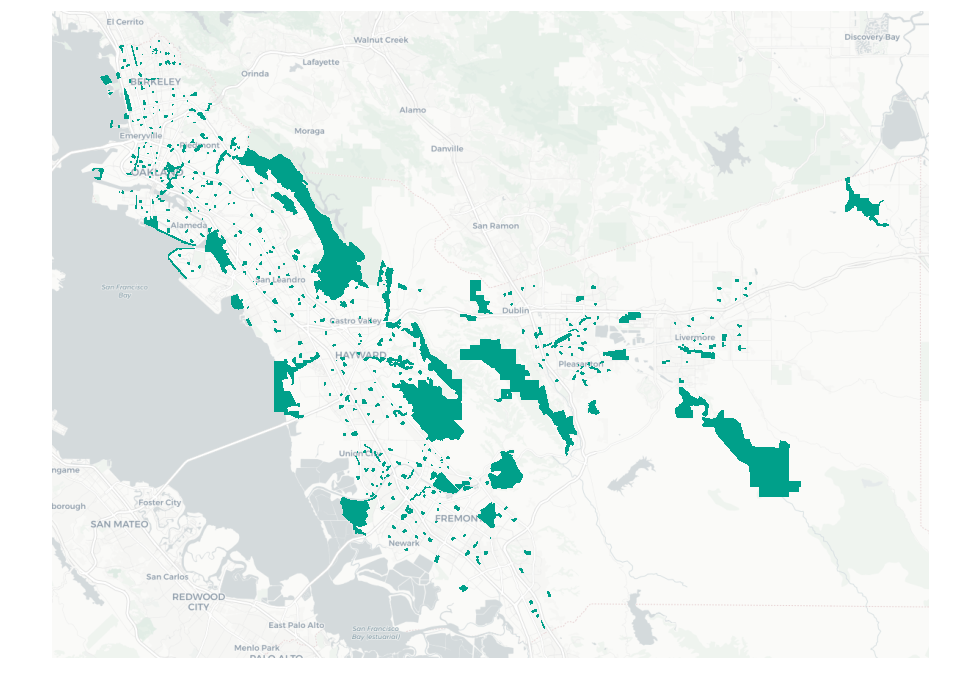
\includegraphics{alameda_destinationchoice_files/figure-latex/parks-map-1.pdf}
\caption{\label{fig:parks-map}Location of parks in Alameda County.}
\end{figure}

We provided the park boundaries layer to a commercial firm, StreetLight Data
Inc., which develops and resells origin-destination matrices derived from
passive device location data. The provider employs a proprietary data processing
engine (called Route Science) to algorithmically transform observed device
location data points (the provider uses in-vehicle GPS units and mobile device
LBS) over time into contextualized, normalized, and aggregated travel patterns.
From these travel patterns, the Route Science processing algorithms infer likely
home Census block group locations for composite groups of people and converts
raw location data points into trip origin and destination points \citep{Pan2006, Friedrich2010}.

For each park polygon, the firm returned a population-weighted estimate of how
many devices were observed by home location block group over several months in
the period between May 2018 and October 2018. We transformed this table such
that it represented the weighted unique devices traveling between block groups
and parks. We discarded home location block groups outside of Alameda County;
the imputed home locations can be far away from the study area for a small
amount of trips and are unlikely to represent common or repeated park
activities. Table \ref{tab:parkstable} presents descriptive statistics on
the 500 parks assembled for this study, grouped according to the
park type as defined on CPAD. A little more than half of the parks have
identified paths, while around 40\% of the identified parks have playgrounds and
sport fields.

\begin{table}

\caption{\label{tab:parkstable}Park Summary Statistics}
\centering
\begin{tabular}[t]{llllll}
\toprule
\multicolumn{2}{c}{ } & \multicolumn{2}{c}{Local Park (N=441)} & \multicolumn{2}{c}{Recreation Area (N=59)} \\
\cmidrule(l{3pt}r{3pt}){3-4} \cmidrule(l{3pt}r{3pt}){5-6}
  &    & Mean & Std. Dev. & Mean  & Std. Dev. \\
\midrule
Acres &  & 59.8 & 370.5 & 125.6 & 505.1\\
Mobile Devices &  & 1450.0 & 6685.4 & 2659.0 & 6161.0\\
\midrule
 &  & N & \% & N & \%\\
type & Local Park & 441 & 100.0 & 0 & 0.0\\
 & Local Recreation Area & 0 & 0.0 & 57 & 96.6\\
 & State Recreation Area & 0 & 0.0 & 2 & 3.4\\
Access & Open Access & 441 & 100.0 & 59 & 100.0\\
 & No Public Access & 0 & 0.0 & 0 & 0.0\\
 & Restricted Access & 0 & 0.0 & 0 & 0.0\\
Playground & FALSE & 213 & 48.3 & 43 & 72.9\\
 & TRUE & 228 & 51.7 & 16 & 27.1\\
Any Sport Field & FALSE & 270 & 61.2 & 38 & 64.4\\
 & TRUE & 171 & 38.8 & 21 & 35.6\\
Football / Soccer & FALSE & 414 & 93.9 & 51 & 86.4\\
 & TRUE & 27 & 6.1 & 8 & 13.6\\
Baseball & FALSE & 363 & 82.3 & 45 & 76.3\\
 & TRUE & 78 & 17.7 & 14 & 23.7\\
Basketball & FALSE & 337 & 76.4 & 52 & 88.1\\
 & TRUE & 104 & 23.6 & 7 & 11.9\\
Tennis & FALSE & 387 & 87.8 & 52 & 88.1\\
 & TRUE & 54 & 12.2 & 7 & 11.9\\
Volleyball & FALSE & 433 & 98.2 & 57 & 96.6\\
 & TRUE & 8 & 1.8 & 2 & 3.4\\
Trail & FALSE & 147 & 33.3 & 21 & 35.6\\
 & TRUE & 294 & 66.7 & 38 & 64.4\\
\bottomrule
\end{tabular}
\end{table}

In order to understand the demographic makeup of the home block groups and
potentially the characteristics of the people who make each trip, we obtained
2013-2017 five-year data aggregations from the American Community Survey using
the \texttt{tidycensus} \citep{Walker2019} interface to the Census API for several key
demographic and built environment variables: the share of individuals by race,
the share of households by income level, household median income, the share of
households with children under 6 years old, and the household density. An
important attribute of the choice model is the distance from the home block
group to the park boundary. Because we have no information on where in the block
group a home is actually located, we use the population-weighted block group
centroid published by the Census Bureau as the location for all homes in the
block group. We then measured the network-based distance between the park and
the home block group centroid using a walk network derived from OpenStreetMap
via the \texttt{networkx} package for Python \citep{networkx},

\begin{table}

\caption{\label{tab:acs-table}Block Group Summary Statistics}
\centering
\resizebox{\linewidth}{!}{
\begin{tabular}[t]{>{\raggedright\arraybackslash}p{4cm}rrrrrrr}
\toprule
  & Unique (\#) & Missing (\%) & Mean & SD & Min & Median & Max\\
\midrule
Density: Households per square kilometer & 1040 & 0 & 1726.3 & 1576.8 & 0.0 & 1373.3 & 21930.9\\
Income: Median tract income & 978 & 3 & 106026.7 & 48909.9 & 13472.0 & 98206.5 & 250001.0\\
Low Income: Share of households making less than \$35k & 977 & 0 & 16.2 & 13.2 & 0.0 & 12.9 & 100.0\\
High Income: Share of households making more than \$125k & 1022 & 0 & 38.6 & 20.8 & 0.0 & 36.9 & 89.2\\
Children: Share of households with children under 6 & 976 & 0 & 14.5 & 8.7 & 0.0 & 13.2 & 48.7\\
Black: Share of population who is Black & 914 & 0 & 11.6 & 14.0 & 0.0 & 6.3 & 80.8\\
Asian: Share of population who is Asian & 1022 & 0 & 26.7 & 20.6 & 0.0 & 20.8 & 93.9\\
Hispanic: Share of population who is Hispanic* & 1031 & 0 & 22.2 & 18.7 & 0.0 & 16.0 & 88.2\\
White: Share of population who is White & 1030 & 0 & 33.5 & 22.5 & 0.0 & 28.8 & 93.6\\
\bottomrule
\multicolumn{8}{l}{\rule{0pt}{1em}\textsuperscript{*} Hispanic indicates Hispanic individuals of all races; non-Hispanic individuals report a single race alone.}\\
\end{tabular}}
\end{table}

\hypertarget{model-application-data}{%
\subsubsection{Model application data}\label{model-application-data}}

We compiled a list of streets in Berkeley, Oakland, and Alameda that were
converted to public open space from each city's respective websites
\citep{city_of_alameda_slow_2020, city_of_oakland_oakland_2020, city_of_berkeley_berkeley_2020} and referred to the ``Shifting Streets'' COVID-19
mobility dataset \citep{slowstreets} to determine whether other cities and places
within Alameda County have similar Open Streets projects (as best as we could
determine, they did not). Based on the information we gathered from these
sources, 74 individual streets were converted; these streets
represent 27.6 total miles across
the cities of Berkeley, Oakland, and Alameda. For the purposes of this analysis,
we represent each opened street as a single ``park'' without any sport facilities
or playgrounds, but with a trail / walking path. The database provides the
opened streets as polyline objects; we assert a 25-foot buffer around the line
to represent a polygon with a measurable area. The 25-foot buffer effectively
counts one vehicle lane and one shoulder parking lane in each direction as
converted to ``park'' space. Finally, we measure the network-based distance from
each population-weighted block group centroid to the nearest boundary of each
new open space facility created by this policy.

\hypertarget{model-estimation}{%
\subsection{Model estimation}\label{model-estimation}}

In random utility choice theory, if an individual living in block group \(n\)
wishes to make a park trip, the probability that the individual will choose park
\(i\) from the set of all parks \(J\) can be described as a ratio of the park's
measurable utility \(V_{ni}\) to the sum of the utilities for all parks in the
set. In the common destination choice framework we apply a multinomial logit
model \citep{McFadden1974, Recker1978},
\begin{equation}\label{eq:p}
   P_{ni} = \frac{\exp(V_{ni})}{\sum_{j \in J}\exp(V_{nj})}
\end{equation}
where the measurable utility \(V_{ni}\) is a linear-in-parameters function of
the destination attributes.
\begin{equation}\label{eq:V}
V_{ni} = X_{ni}\beta
\end{equation}
where \(\beta\) is a vector of estimable coefficients giving the relative utility
(or disutility) of that attribute to the choice maker, all else equal. It is
possible to add amenities of the park or the journey to the utility equation.
However, as the number of alternatives is large, it is impractical to consider
alternative-specific constants or coefficients and therefore not possible to
include attributes of the home block group or traveler \(n\) directly. We can,
however, segment the data and estimate distinct distance and size parameters
for different segments to observe heterogeneity in the utility parameters
between different socioeconomic groups.

The logarithm of the sum in the denominator of Equation \ref{eq:p} (called the
logsum) provides a measure of the consumer surplus of the choice set enjoyed by
person \(n\) \citep{Williams1977a},
\begin{equation}
CS_n = \ln{{\sum_{j \in J}\exp(V_{nj})}} + C
  \label{eq:logsum}
\end{equation}
where \(C\) is a constant indicating an unknown absolute value; the difference of
logsum values in two different scenarios eliminates \(C\). Additionally, dividing
the difference in logsum from choice set \(J\) and choice set \(J'\) by a cost
coefficient \(\beta\)
\begin{equation}
\delta CS_n = (\ln{\sum_{j \in J'}\exp(V_{nj})} - \ln{\sum_{j \in J}\exp(V_{nj})})/\beta
  \label{eq:deltalogsum}
\end{equation}
gives an estimate of the benefit received by person \(n\) in monetary terms. Thus,
such a ``utility-based'' accessibility term is continuously defined, contains
multiple dimensions of the attributes of the choice, and can be evaluated in
monetary terms \citep{Handy1997, Dong2006}. Note also that the logsum increases
with the size of the choice set: if a new alternative \(q\) is added to \(J\), then
\(\ln\sum_{j\in J}\exp(V_j) < \ln(\sum_{j\in J}\exp(V_j) + \exp(V_q))\) for
any value of \(V_q\).

In the most typical cases, researchers estimate the utility coefficients for
destination choice models from household travel surveys. For example, the
California add-on to the 2017 National Household Travel Survey could be used for
this purpose for frequent trips like commutes to work and school. However, as a
24-hour trip diary, it is less useful for recreational trips that may take place
less frequently. For better data on park access, we need to synthesize a
suitable estimation data set. We do this by sampling 20,000 random discrete
device origin-destination pairs from the commercial passive data matrix,
weighted by the volume of the flows. This corresponds to a
4.3\% sample of all the observed device
origin-destination pairs.

The sampled origin-destination pair gives the home location as well as the
``chosen'' alternative for a synthetic person. In principle the individual's
choice set contains all the parks in our dataset; in practice it can be
difficult to estimate choice models with so many alternatives (\(|J| = 500\)).
For this reason we randomly sample 10 additional parks
to serve as the non-chosen alternatives, with a different set of 10 parks for
each synthetic choice maker. Such
random sampling of alternatives reduces the efficiency of the estimated
coefficients but the coefficients remain unbiased \citep{train2009}; a more elegant
sampling approach might have resulted in smaller estimated standard errors,
but the estimation results (presented below) suggest this is not a concern in
this application. As the model has
no alternative-specific constants, the standard likelihood comparison statistic
against the market shares model \(\rho^2\) is not computable. We instead use the
likelihood comparison against the equal shares model \(\rho_0^2\).

The resulting analysis dataset therefore contains 20,000 choice makers that
select between 11 parks including the park they were observed to
choose; the measured distance between the choice maker's block group and all
parks in the choice set; and the acreage of each park in the choice set. We use
the \texttt{mlogit} package for R \citep{mlogit, R} to estimate the multinomial logit
models.

\hypertarget{model-application}{%
\subsection{Model application}\label{model-application}}

Using the full set of Alameda County parks --- including those added by street
conversion --- we can apply a destination choice model to calculate the change in
park choice utilities and utility-based accessibility values for each block
group in Alameda County. As shown with Equation \eqref{eq:deltalogsum}, the
difference in utility-based accessibility values with and without the opened
streets is the additional consumer surplus provided by the policy, converted into a
monetary value by a cost-utility coefficient. The purpose of converting the logsum
into a monetary value is to scale the benefits in terms that analysts and
policy makers can compare
more easily than raw utility values. The dataset used for this research
does not have any information on travel costs or entrance fees, and such data
would likely not be relevant in the context of urban parks. As a result, there
is no direct link between the utility and a monetary cost in our estimated
models.

As a substitution, we use an estimate of the cost coefficient obtained from the
Metropolitan Transportation Commission (MTC, San Francisco Bay regional MPO)
``Travel Model One'' activity-based travel demand model \citep{mtctm1}. In this model,
the utility of destination choice for social and recreational trips uses
the mode choice model logsum as an impedance measure.
The mode choice model cost coefficient varies with each individual's value of time.
The average value of time in the synthetic population for the calibration
scenario is \$7.75 per hour. Dividing that value of time by the in-vehicle
travel time parameter of \(-0.018\) results in an implied mode choice cost coefficient of
\((-0.018 /min * 60 min / hr)/ (7.75 \$/hr) = -0.139 / \$\).

\hypertarget{results}{%
\section{Results}\label{results}}

We estimated multinomial logit park activity location choice models on the
datset described in the previous section. We applied a Yeo-Johnson
transformation \citep{Yeo2000} to both the walk distance (in meters) between the
park and the block group centroid, and to the park acreage. The Yeo-Johnson
transformation replicates the constant marginal elasticity of a logarithmic
transformation while avoiding undefined values (e.g., \(YJ(0) = 0\)). For
simplicity, we call this transformation \(\log()\) in the model results tables.
Using a constant marginal elasticity is better reflective of how people perceive
distances and sizes; a one-mile increase to a trip distance matters more to a
two-mile trip than a ten-mile trip.

Table \ref{tab:base-modelsummary} presents the model estimation results for
each estimated model. The ``Network Distance'' model, which only considers the
distance to the park and the size of the park. results in significant estimated
coefficients of the expected sign. That is, individuals will travel further
distances to reach larger parks. The ratio of the estimated coefficients implies
that on average, people will travel twice as far to reach a park 3.47
times as large.

Table \ref{tab:base-modelsummary} also shows the results of the ``Park
Attributes'' model, which represents the presence of any sport field with a
single dummy variable, and the ``Sport Detail'' model, which disaggregates this
variable into facilities for different sports. The value of the size and
distance coefficients change modestly from the ``Network Distance'' model, with
the implied size to distance trade-off rising to 4.16. Examining
the two amenities models --- independently and in comparison with each other ---
reveals a few surprising findings. First, it appears that playgrounds and sport
fields in general contribute \emph{negatively} to the choice utility equation. This
is both unintuitive and contradictory to previous findings in this space \citep[e.g.,][]{Kinnell2006}. Considering different sports separately, there is a wide variety
of observed response with tennis and volleyball facilities attracting more
trips, and football and basketball facilities attracting fewer, all else equal.
Trails and walking paths give substantive positive utility in both models. The
difference in likelihood statistics between the three models is significant
(likelihood ratio test between Sport Detail and Park Attributes model has
\(p\)-value 2.68e-06), and so in spite of the curious aggregate findings,
we move forward with this utility specification.

\begin{table}

\caption{\label{tab:base-modelsummary}Estimated Model Coefficients}
\centering
\begin{tabular}[t]{lccc}
\toprule
  & Network Distance & Park Attributes & Sport Detail\\
\midrule
log(Distance) & -1.358 *** & -1.397 *** & -1.389 ***\\
 & (0.010) & (0.010) & (0.010)\\
log(Acres) & 0.391 *** & 0.337 *** & 0.334 ***\\
 & (0.005) & (0.005) & (0.005)\\
Playground &  & -0.448 *** & -0.556 ***\\
 &  & (0.022) & (0.022)\\
Trail &  & 0.576 *** & 0.592 ***\\
 &  & (0.024) & (0.024)\\
Sport Field &  & -0.381 *** & \\
 &  & (0.023) & \\
Basketball &  &  & -0.293 ***\\
 &  &  & \vphantom{2} (0.030)\\
Baseball &  &  & 0.130 ***\\
 &  &  & \vphantom{1} (0.030)\\
Football / Soccer &  &  & -0.467 ***\\
 &  &  & (0.042)\\
Tennis &  &  & 0.202 ***\\
 &  &  & (0.030)\\
Volleyball &  &  & 0.125 *\\
 &  &  & (0.061)\\
Other Sport &  &  & -0.249 ***\\
 &  &  & (0.039)\\
\midrule
Num.Obs. & 20,000 & 20,000 & 20,000\\
AIC & 58,736.3 & 57,014.9 & 56,991.2\\
Log Likelihood & -29,366.1 & -28,502.5 & -28,485.6\\
\$\textbackslash{}rho\textasciicircum{}2\_0\$ & 0.388 & 0.406 & 0.406\\
\bottomrule
\multicolumn{4}{l}{\textsuperscript{} Standard errors in parentheses.}\\
\end{tabular}
\end{table}

It is worth investigating the heterogeneity in preferences that exist among
populations. Though the income and ethnicity of the synthetic park visitors is
not known, we can segment the estimation dataset based on the socioeconomic
makeup of the visitors' residence block group. The models presented in Table
\ref{tab:grouped-modelsummary} were estimated on segments developed in this
manner. Models under the ``Race/Ethnicity'' heading include a race- and
ethnicity-based segmentation: simulated individuals living in block groups with
more than thirty percent Black residents are included in the ``\textgreater30\% Black'' model,
an analogous segmentation for block groups with high Asian and Hispanic
populations are in the ``\textgreater30\% Asian'' and ``\textgreater30\% Hispanic'' models respectively, and
the ``Other'' model contains all other block groups. Another set of model
segmentation relies on the share of the population in each block group with
household incomes above or below certain thresholds, and a third relies on the
share of households with children under 6 years old. Again, we use the threshold
definitions largely informed by the distributions in Table \ref{tab:acs-table}.

\begin{landscape}\begin{table}

\caption{\label{tab:grouped-modelsummary}Estimated Model Coefficients with Block Group Segmentations}
\centering
\resizebox{\linewidth}{!}{
\begin{tabular}[t]{lcccccccccc}
\toprule
\multicolumn{1}{c}{ } & \multicolumn{4}{c}{Race/Ethnicity} & \multicolumn{3}{c}{Income} & \multicolumn{3}{c}{Children} \\
\cmidrule(l{3pt}r{3pt}){2-5} \cmidrule(l{3pt}r{3pt}){6-8} \cmidrule(l{3pt}r{3pt}){9-11}
  & > 30\% Asian & > 30\% Black & > 30\% Hispanic & Other Eth. & > 30\% Low income & > 50\% High income & Other Inc. & > 25\% Children & < 5\% Children & Other Children\\
\midrule
\cellcolor{gray!6}{log(Distance)} & \cellcolor{gray!6}{-1.278 ***} & \cellcolor{gray!6}{-1.515 ***} & \cellcolor{gray!6}{-1.268 ***} & \cellcolor{gray!6}{-1.492 ***} & \cellcolor{gray!6}{-1.418 ***} & \cellcolor{gray!6}{-1.392 ***} & \cellcolor{gray!6}{-1.360 ***} & \cellcolor{gray!6}{-1.271 ***} & \cellcolor{gray!6}{-1.561 ***} & \cellcolor{gray!6}{-1.387 ***}\\
 & (0.017) & (0.030) & (0.022) & (0.019) & (0.026) & (0.020) & (0.013) & (0.029) & (0.037) & (0.011)\\
\cellcolor{gray!6}{log(Acres)} & \cellcolor{gray!6}{0.368 ***} & \cellcolor{gray!6}{0.262 ***} & \cellcolor{gray!6}{0.323 ***} & \cellcolor{gray!6}{0.340 ***} & \cellcolor{gray!6}{0.310 ***} & \cellcolor{gray!6}{0.360 ***} & \cellcolor{gray!6}{0.329 ***} & \cellcolor{gray!6}{0.339 ***} & \cellcolor{gray!6}{0.366 ***} & \cellcolor{gray!6}{0.332 ***}\\
 & (0.009) & (0.015) & (0.011) & (0.010) & (0.014) & (0.010) & (0.007) & (0.014) & (0.020) & (0.006)\\
\cellcolor{gray!6}{Playground} & \cellcolor{gray!6}{-0.458 ***} & \cellcolor{gray!6}{-0.639 ***} & \cellcolor{gray!6}{-0.327 ***} & \cellcolor{gray!6}{-0.780 ***} & \cellcolor{gray!6}{-0.593 ***} & \cellcolor{gray!6}{-0.621 ***} & \cellcolor{gray!6}{-0.520 ***} & \cellcolor{gray!6}{-0.344 ***} & \cellcolor{gray!6}{-0.670 ***} & \cellcolor{gray!6}{-0.579 ***}\\
 & (0.038) & (0.060) & (0.047) & (0.042) & (0.055) & (0.045) & (0.029) & (0.062) & (0.078) & (0.025)\\
\cellcolor{gray!6}{Trail} & \cellcolor{gray!6}{0.533 ***} & \cellcolor{gray!6}{0.574 ***} & \cellcolor{gray!6}{0.280 ***} & \cellcolor{gray!6}{0.970 ***} & \cellcolor{gray!6}{0.573 ***} & \cellcolor{gray!6}{0.840 ***} & \cellcolor{gray!6}{0.527 ***} & \cellcolor{gray!6}{0.360 ***} & \cellcolor{gray!6}{0.731 ***} & \cellcolor{gray!6}{0.610 ***}\\
 & (0.041) & (0.062) & (0.049) & (0.049) & (0.058) & (0.054) & (0.031) & (0.064) & (0.087) & (0.027)\\
\cellcolor{gray!6}{Basketball} & \cellcolor{gray!6}{-0.170 ***} & \cellcolor{gray!6}{-0.255 **} & \cellcolor{gray!6}{-0.503 ***} & \cellcolor{gray!6}{-0.411 ***} & \cellcolor{gray!6}{-0.230 **} & \cellcolor{gray!6}{-0.193 ***} & \cellcolor{gray!6}{-0.390 ***} & \cellcolor{gray!6}{-0.445 ***} & \cellcolor{gray!6}{-0.359 **} & \cellcolor{gray!6}{-0.261 ***}\\
 & (0.049) & (0.085) & (0.067) & (0.060) & (0.077) & (0.058) & (0.041) & (0.083) & (0.110) & (0.034)\\
\cellcolor{gray!6}{Baseball} & \cellcolor{gray!6}{0.097 *} & \cellcolor{gray!6}{0.200 *} & \cellcolor{gray!6}{0.148 *} & \cellcolor{gray!6}{0.163 **} & \cellcolor{gray!6}{0.226 **} & \cellcolor{gray!6}{-0.023} & \cellcolor{gray!6}{0.187 ***} & \cellcolor{gray!6}{0.162 *} & \cellcolor{gray!6}{0.153} & \cellcolor{gray!6}{0.125 ***}\\
 & (0.049) & (0.080) & (0.063) & (0.058) & (0.073) & (0.060) & (0.039) & (0.080) & (0.107) & (0.033)\\
\cellcolor{gray!6}{Football / Soccer} & \cellcolor{gray!6}{-0.282 ***} & \cellcolor{gray!6}{-0.731 ***} & \cellcolor{gray!6}{-0.595 ***} & \cellcolor{gray!6}{-0.630 ***} & \cellcolor{gray!6}{-0.689 ***} & \cellcolor{gray!6}{-0.178 *} & \cellcolor{gray!6}{-0.588 ***} & \cellcolor{gray!6}{-0.357 **} & \cellcolor{gray!6}{-0.514 ***} & \cellcolor{gray!6}{-0.482 ***}\\
 & (0.065) & (0.125) & (0.100) & (0.084) & (0.104) & (0.080) & (0.058) & (0.116) & (0.147) & (0.048)\\
\cellcolor{gray!6}{Tennis} & \cellcolor{gray!6}{0.417 ***} & \cellcolor{gray!6}{-0.428 ***} & \cellcolor{gray!6}{-0.067} & \cellcolor{gray!6}{0.305 ***} & \cellcolor{gray!6}{-0.211 **} & \cellcolor{gray!6}{0.560 ***} & \cellcolor{gray!6}{0.120 **} & \cellcolor{gray!6}{0.162 +} & \cellcolor{gray!6}{0.131} & \cellcolor{gray!6}{0.213 ***}\\
 & (0.047) & (0.096) & (0.070) & (0.056) & (0.082) & (0.055) & (0.040) & (0.084) & (0.107) & (0.033)\\
\cellcolor{gray!6}{Volleyball} & \cellcolor{gray!6}{0.080} & \cellcolor{gray!6}{-0.222} & \cellcolor{gray!6}{0.122} & \cellcolor{gray!6}{0.244 *} & \cellcolor{gray!6}{-0.184} & \cellcolor{gray!6}{0.286 **} & \cellcolor{gray!6}{0.009} & \cellcolor{gray!6}{-0.116} & \cellcolor{gray!6}{0.121} & \cellcolor{gray!6}{0.163 *}\\
 & (0.096) & (0.225) & (0.141) & (0.106) & (0.195) & (0.100) & (0.087) & (0.173) & (0.247) & (0.068)\\
\cellcolor{gray!6}{Other Sport} & \cellcolor{gray!6}{-0.171 **} & \cellcolor{gray!6}{-0.297 *} & \cellcolor{gray!6}{-0.418 ***} & \cellcolor{gray!6}{-0.303 ***} & \cellcolor{gray!6}{-0.521 ***} & \cellcolor{gray!6}{-0.170 *} & \cellcolor{gray!6}{-0.250 ***} & \cellcolor{gray!6}{-0.220 *} & \cellcolor{gray!6}{-0.353 *} & \cellcolor{gray!6}{-0.244 ***}\\
 & (0.061) & (0.116) & (0.095) & (0.073) & (0.107) & (0.073) & (0.052) & (0.109) & (0.139) & (0.044)\\
\midrule
\cellcolor{gray!6}{Num.Obs.} & \cellcolor{gray!6}{6,861} & \cellcolor{gray!6}{2,600} & \cellcolor{gray!6}{3,790} & \cellcolor{gray!6}{6,749} & \cellcolor{gray!6}{2,982} & \cellcolor{gray!6}{5,759} & \cellcolor{gray!6}{11,259} & \cellcolor{gray!6}{2,365} & \cellcolor{gray!6}{1,769} & \cellcolor{gray!6}{15,866}\\
AIC & 20,513.9 & 7,675.8 & 12,386.6 & 15,939.9 & 9,070.6 & 14,438.9 & 33,286.6 & 7,646.5 & 4,526.1 & 44,789.2\\
\cellcolor{gray!6}{Log Likelihood} & \cellcolor{gray!6}{-10,247} & \cellcolor{gray!6}{-3,827.9} & \cellcolor{gray!6}{-6,183.3} & \cellcolor{gray!6}{-7,960} & \cellcolor{gray!6}{-4,525.3} & \cellcolor{gray!6}{-7,209.5} & \cellcolor{gray!6}{-16,633.3} & \cellcolor{gray!6}{-3,813.3} & \cellcolor{gray!6}{-2,253} & \cellcolor{gray!6}{-22,384.6}\\
\$\textbackslash{}rho\textasciicircum{}2\_0\$ & 0.377 & 0.386 & 0.320 & 0.508 & 0.367 & 0.478 & 0.384 & 0.328 & 0.469 & 0.412\\
\bottomrule
\multicolumn{11}{l}{\textsuperscript{} Standard errors in parentheses.}\\
\multicolumn{11}{l}{\textsuperscript{a} Simulated individuals segmented based on the share of households meeting the segmentation threshold in the residence block group.}\\
\end{tabular}}
\end{table}
\end{landscape}

The model estimates in Table \ref{tab:grouped-modelsummary} reveal noticeable
heterogeneity in the park location choices among visitors from different block
group segments. Park visitors living in block groups with a high proportion of
Black and low-income residents show less affinity for trails and other walkways,
but appear considerably more sensitive to the distance to a park. Park visitors
living in high-income neighborhoods are less sensitive to the distance to a
park, but receive more utility from certain amenities, in particular trails and
tennis courts. Block groups with a high proportion of Hispanic residents and
residents with children under 6 show the least negative response to playgrounds
of all the segments.

Seeing that there is a difference in the response in the model segmentation, it
is also worth considering the role of our segmentation thresholds in these
findings. Figure \ref{fig:split-plots} shows the estimated coefficients and
confidence intervals for these different amenities at different threshold levels
of segmentation. The threshold level means that at least that percent of the
block group's population falls in that category. The confidence intervals widen
as more observations are excluded from the model. The estimated coefficients for
the different segmentations are identical when the share equals zero, and simply
represent the ``Sport Detail'' model from Table \ref{tab:base-modelsummary}.

Overall, increasing the segmentation threshold level reveals additional
information about user preferences. First, it should be noted that there is some
inconsistency: for instance, block groups with at least 30\% of low income
households show a lower importance of distance than block groups with either 20\%
or 40\% low income households, though all three estimates are within the same
confidence intervals. The increasing width of the confidence interval, however,
means it is sometimes difficult to make robust statements. Residents of
block groups with a higher share of Asian individuals or high income households both show
relatively more affinity for tennis courts and trails relative to other groups.
Residents of block groups with increasing shares of Hispanic individuals show
the highest affinity for playgrounds, and park goers from neighborhoods with a
greater share of Black individuals are most sensitive to distance and least
sensitive to park size.

\begin{figure}
\centering
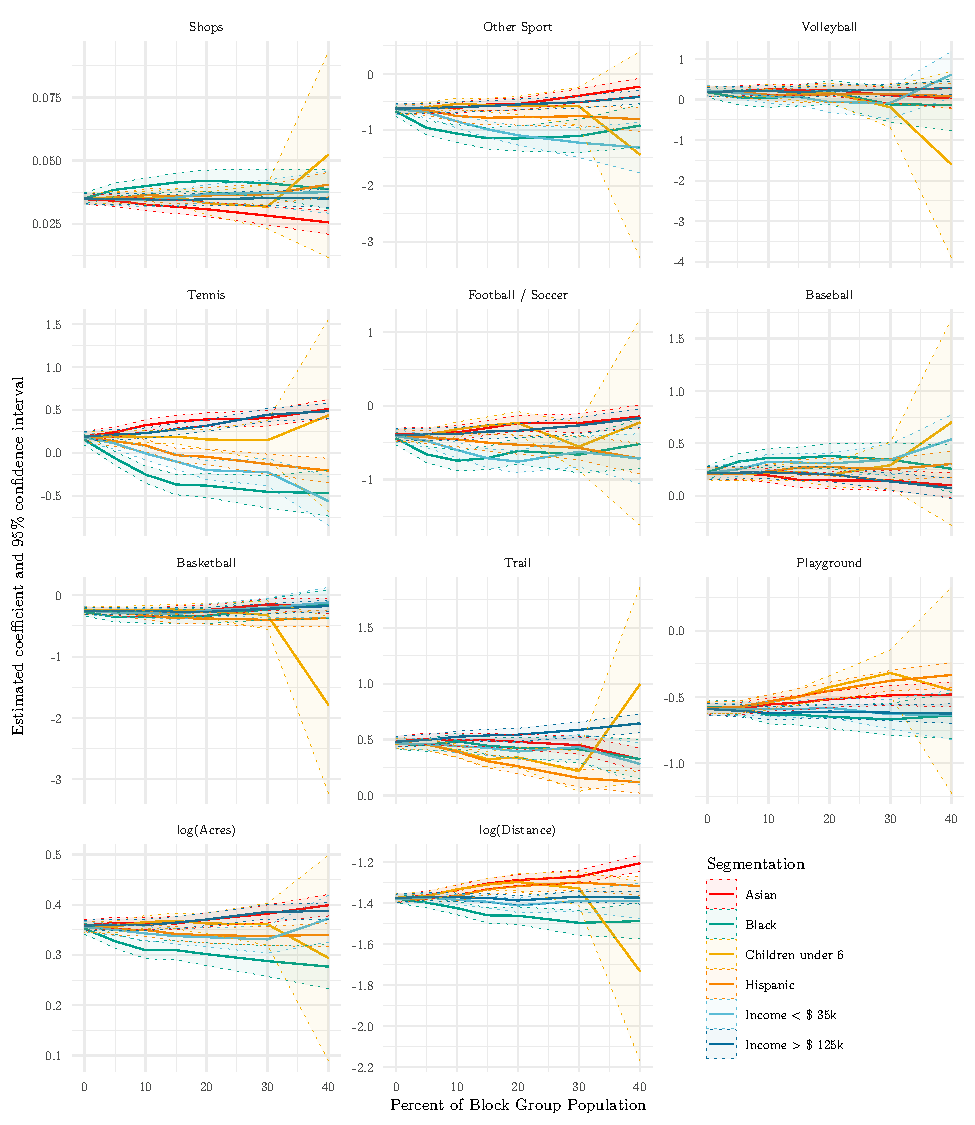
\includegraphics{alameda_destinationchoice_files/figure-latex/split-plots-1.pdf}
\caption{\label{fig:split-plots}Estimated utility coefficients and 95\% confidence intervals for park amenities at different socioeconomic threshold levels.}
\end{figure}

\hypertarget{equity-analysis-of-covid-19-street-openings}{%
\subsection{Equity Analysis of COVID-19 Street Openings}\label{equity-analysis-of-covid-19-street-openings}}

In this section, we apply the models estimated above to evaluate the benefits of
the street conversion policy in terms of aggregate value determined by the
change in accessibility logsum, as well as the equity of the policy with respect
to different income and ethnic groups. In this analysis, we apply the ``Sport Detail''
non-segmented model from Table \ref{tab:base-modelsummary}, as it had the best
fit of these models.

Figure \ref{fig:logsumsmap} presents this monetary valuation spatially.
Unsurprisingly, the benefits are concentrated in the block groups surrounding
the opened streets. Most residents of central Oakland see a benefit of somewhere
around \$1, while some zones see an equivalent benefit of as much as \$30. One
property of logsum-based accessibility terms is that there is some benefit given
for simply having more options, whether or not those options are attractive in
any way. In this application, these benefits are small, on the order of 10 cents
for most block groups away from where the street openings occurred.

\begin{figure}
\centering
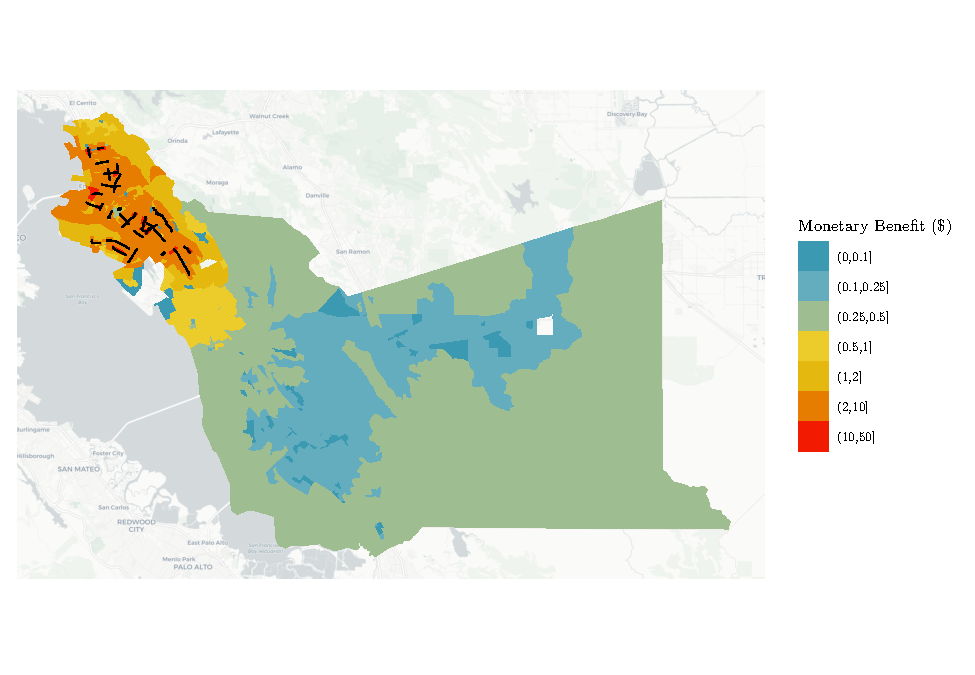
\includegraphics{alameda_destinationchoice_files/figure-latex/logsumsmap-1.pdf}
\caption{\label{fig:logsumsmap}Monetary value of street opening to residents based on utility change. Streets converted to pedestrian plazas are shown in black.}
\end{figure}

More interesting than the total benefit or even its spatial distribution,
however, is the social equity of its distribution among different population
segments. If we assign the block-group level monetary benefit to each household
in the block group, we can begin to allocate the distribution of benefits
proportionally to households of different sociodemographic classifications.
Specifically, if a block group with \(N\) total households has a measured consumer
surplus \(\delta CS\), then the share of the total benefits going to a particular
population segment \(k\) is

\begin{equation}
  S_k = N * P_k * \delta CS
  \label{eq:cs-alloc}
\end{equation}

where \(P_k\) is the proportion of the block group's population in segment \(k\).
There is some opportunity for confusion when some demographic variables we use
(share of households with children, household income) are defined at the
household level and others (specifically ethnicity) are defined at the person level. It is
similarly not clear whether the benefits of improved park access should be
assigned at the person level, the household level, or the number of total park
trip makers in each block group. For consistency and simplicity, we assert that
the benefit is assigned to each household, and that persons receive a
proportional share of the household benefit. For example, a block group with 30\%
Black individuals will receive 30\% of the benefits assigned to all the
households in the block group.

Table \ref{tab:equity} shows the total benefit assigned to households in this
way as well as the share of all monetary benefits in the region. In some cases,
the policy of opening streets as public spaces had a pro-social benefit, as
18.7\% of benefits went to Black individuals, even though only 11.4\% of the
population of Alameda County is Black. Similarly, roughly one-quarter of total
benefits went to households making less than \$35,000 per year even though only
one-fifth of the households are in this category. On the other hand, a smaller
than expected share of benefits is allocated to Asian individuals and households
making more than \$125,000 per year.

\begin{table}

\caption{\label{tab:equity}Equity Distribution of Street Opening Benefits}
\centering
\resizebox{\linewidth}{!}{
\begin{tabular}[t]{>{\raggedright\arraybackslash}p{1.8in}>{\centering\arraybackslash}p{1in}>{\centering\arraybackslash}p{1in}>{\centering\arraybackslash}p{1in}>{\centering\arraybackslash}p{1in}}
\toprule
Group & Benefit & Percent* of Benefits & Households** & Percent of Households\\
\midrule
Households with Children under 6 & \$145,604 & 14.10 & 83,868 & 14.53\\
Income < \$35k & \$223,853 & 21.68 & 90,762 & 15.73\\
Income > \$125k & \$329,431 & 31.91 & 229,963 & 39.84\\
Black & \$187,483 & 18.16 & 61,971 & 10.74\\
Asian & \$199,032 & 19.28 & 167,135 & 28.96\\
\addlinespace
Hispanic & \$230,674 & 22.34 & 119,013 & 20.62\\
White & \$351,749 & 34.07 & 194,263 & 33.66\\
All Households & \$1,032,372 & 100.00 & 577,177 & 100.00\\
\bottomrule
\multicolumn{5}{l}{\rule{0pt}{1em}\textsuperscript{*} As individuals and households will belong in multiple groups, the percents do not sum to 100.}\\
\multicolumn{5}{l}{\rule{0pt}{1em}\textsuperscript{\dag} Race and ethnicity are person-level attributes; households are assumed to follow the same distribution.}\\
\end{tabular}}
\end{table}

\hypertarget{limitations}{%
\section{Limitations and Future Directions}\label{limitations}}

The utility-based accessibility metrics we present and apply in this paper are
evaluated from a discrete choice model estimated on simulated decision makers
constructed from a third-party passive origin-destination matrix. This
methodological choice has some strengths: Foremost among these is the ability to
readily and affordably construct a large dataset on an infrequent trip purpose.
Most destination choice and activity location models are estimated on
small-sample household travel surveys. Securing sufficient responses to estimate
a rich behavioral model on a trip purpose as infrequent as parks has proven
prohibitively expensive outside of extensive research activities \citep[e.g.,][]{Kaczynski2016}. Using passive data sets to increase the effective sampling rate
possible in a discrete choice model is a potentially powerful strategy, and its
application here is an important contribution of our work.

At the same time, passive data sets available from commercial providers do not
reveal any details about the specific trip makers beyond what can be learned
from their residence block group. In this research we were able to determine
whether a device resided in a block group with a high proportion of low-income
households, but could not have confidence that a particular device belonged to a
member of such a household. Similarly, there is no information on what kind of
trip the device-holder actually accomplished at each park. These limitations
combined mean that it would likely be infeasible to directly observe devices
that traveled to the converted streets during the COVID-19 lockdowns. The ideal
dataset for estimating individual park activity location choices generally and
in special situations remains a high-quality, large-sample household survey of
real individuals.

The individual-level demographic data would also be valuable in understanding
more clearly the observed heterogeneity in response among different income or
ethnic groups. The trends and correlations revealed in the presented models may
reflect situational inequities rather than true preferences. For example, the
distinct observed parameters on size and distance for block groups with high
minority populations may indicate that areas with large minority populations
tend to have smaller parks that are more geographically distributed relative to
other areas of the region. This interpretation could also explain some of the
non-intuitive response observed in our models, especially in regards to
playgrounds.

We limited our analysis to home locations and parks in Alameda County,
California. It is possible that some Alameda residents visit parks in
neighboring counties, just as it is possible that parks in Alameda County
attract trips from outside the county borders. This is most likely for block
groups and parks on the north and south borders of the county. The scope of this
analysis was determined by the passive data set available for the research, but
the county boundaries are not a general requirement for all studies of this
kind.

The distance to a park was represented in this study using a walk network
retrieved from the OpenStreetMap project. Though perhaps superior to a Euclidean
distance, this measure still has many limitations. First, we were unable to
verify the integrity of the underlying network information; based on our prior
experience, it is likely that some broken or improperly connected links
artificially inflated the measured distance for an unknown number of park /
block group pairs. A more serious limitation, however, is that experienced
travel distances are a function of the transport mode employed by the traveler.
Using bare distances does not provide any detail on how access to parks might be
increased with improved transit service, for example. Using a mode-choice model
logsum as a multi-modal impedance term in the activity location choice model
would enable this kind of analysis.

The monetary benefits we present in this analysis are heavily dependent on
two separate assumptions. First, reasonable researchers might have selected
different values of time or cost coefficients. Second, the decision to assign
one benefit to each household could also have been made
differently. A change in either assumption would lead to a highly different
total benefits estimate, but it would not change the distribution of the
benefits, which is the objective of this study. At some level, converting the
esoteric measure of choice model logsums into a unit that can be conveniently
compared against other policies is desirable to help the public and policy
makers evaluate such decisions. Further research should establish guidelines and
practices for applying accessibility logsums in monetary cost-benefit analyses.

Of course, COVID-19 led to the closure of some park facilities --- playgrounds,
pavilions, and in some cases entire parks --- that were not captured in this
analysis. These closures would lead to a decrease in the consumer surplus for
park access, which might overwhelm or at least change the distribution of
positive benefits we measured here.

\hypertarget{conclusions}{%
\section{Conclusions}\label{conclusions}}

Converting city roadways into pedestrian-oriented public spaces was in some ways
an obvious response to the COVID-19 pandemic: Vehicle traffic demand was down,
and there was a also critical need for pedestrian-oriented open spaces in many
communities. The research we present here suggests that this policy had
measurable and meaningful benefits to neighborhoods in Alameda County,
California, and that these benefits were distributed in an equitable manner in the sense that the distributin favored marginalized populations. The total benefit to households in the community is estimated
at approximately \$1 million with disproportionately high benefits going to
Black, Hispanic and low-income neighborhoods. There is, however, a
disproportionately low benefit to neighborhoods with high Asian populations that
might be addressed were the policy to continue, be repeated, or made permanent
in some way.

In estimating these benefits, we applied an emerging technique to estimate park
choice preferences and utility from passive mobile device data. This technique
allowed a more nuanced measure of access that allowed us to consider the
converted streets as providing quantitatively different amenities than other city
parks. A policy of permanently closing these streets to vehicle traffic may or
may not have negative effects on transportation access that would need to be
considered against the benefits we measured in this research. But utility-based
access measures provide a mechanism to weigh the benefits of access against the
costs of travel in a theoretically coherent manner. Adopting such flexible
methods of measuring access will help transportation and land use planners
better understand the nuances and tradeoffs inherent in a wide range of policy
proposals.

\hypertarget{acknowledgments}{%
\section*{Acknowledgments}\label{acknowledgments}}
\addcontentsline{toc}{section}{Acknowledgments}

Graphics and tables were developed using several open-source R packages
\citep{ggspatial, modelsummary, wesanderson}.

\bibliography{book.bib}


\end{document}
